% \documentclass{article}
% \usepackage[margin=1cm]{graphicx} % Required for inserting images
% \usepackage[russian]{babel}
% \usepackage{caption}
% \usepackage{geometry}
% \usepackage{url}
% \usepackage{amsfonts}
% \usepackage{amsmath}
% \usepackage{float}
% \usepackage[a4paper, top=2cm, bottom=3cm, left=3cm, right=1cm]{geometry}
\documentclass[a4paper,12pt]{article}
\usepackage[utf8]{inputenc}
\usepackage[russian]{babel}
\usepackage{amsmath}
\usepackage{multicol}
\usepackage{url}
\usepackage[margin=1cm]{graphicx} % Required for inserting images
\usepackage[a4paper, top=2cm, bottom=3cm, left=1cm, right=2cm]{geometry}

\title{Санкт-Петербургский политехнический университет
Петра Великого
Физико-механический институт
Высшая школа прикладной математики и вычислительной
физики}
\date{}
\begin{document}

\maketitle
\begin{center}
{\fontsize{25}{}\selectfont Отчёт \\
по лабораторной работе №3 \\
по дисциплине \\
«Интервальный анализ»}

\end{center}
\begin{flushright}
Выполнил студент:\\
Басалаев Даниил \\
группа:\\
5030102/10201\\

\end{flushright}

\vspace*{\fill} \begin{center}Санкт-Петербург\end{center}

\newpage % Начать новую страницу для содержания
\tableofcontents
\newpage

\section{Теоретическое обоснование}
\textbf{Необходимые формулы:}
\begin{itemize}
\item Выборочная медиана
 \begin{equation*}
 med \text{ } x=\begin{cases} 
    x_{(l+1)}      & \quad \text{при } n = 2l+1 \\
    \frac{x_{(l)}+x_{(l+1)}}{2} & \quad \text{при } n = 2l 
  \end{cases}
 \end{equation*}
    \item \textit{Ширина интервала}
    \begin{equation*}
    wid \textbf{ }a=\overline{\textbf{a}}-\underline{\mathbf{a}}
    \end{equation*}
 \item \textit{Минимум по включению}
    \begin{equation*}
    a \wedge b := \inf_{\subseteq} \{a,b\} = [max\{\underline{a},\underline{b}\}, min \{\overline{a},\overline{b}\}]
    \end{equation*}
    \item \textit{Максимум по включению}
    \begin{equation*}
    a \vee b := \sup_{\subseteq} \{a,b\} = [min\{\underline{a},\underline{b}\}, max \{\overline{a},\overline{b}\}]
    \end{equation*}
    \item \textit{Радиус интервала}
    \begin{equation*}
 rad \textbf{ a}=(\overline{\textbf{a}}-\textbf{\underline{a}})/2
 \end{equation*}

\item \textit{Интервальная мода}:\\
Пусть имеется интервальная выборка\\
$X = \lbrace x_i \rbrace$
Сформируем массив интервалов z из концов интервалов X.
\\Для каждого интервала $z_i$ подсчитываем число $\mu _i$ интервалов из выборки $X_i$, включающих $z_i$. Максимальные $\mu _i$ = max $\mu$ достигаются для индексного множества K. Тогда можно найти
интервальную моду как мультиинтервал\\
mode X = $\bigcup_{k \in K}{z_k}$

\item \textit{Интервальная медиана Крейновича}:\\
Пусть дана выборка X = {$x_i$}. Пусть $\underline{c}$ = {$\underline{x_i}$}, $\overline{c}$ = {$\overline{x_i}$} — конфигурация точек, составленные, соответственно, из левых и правых концов интервалов из X. Медиана Крейновича $med_{K}X$ интервальной выборки X — это интервал\\ $med_K$ = [$med_{\underline{c}}$, $med_{\overline{c}}$].

\item \textit{Интервальная медиана Пролубникова}:\\
Зададим отношения порядка на алгебре $\mathbb{R}$. Говорят, что неравенство $a \leq b$ выполняется\\
\begin{enumerate}
    \item в сильном смысле, если $\forall a \in \mathbb{R}$ $ \forall b \in \mathbb{R}$ : $\overline{a} \leq \underline{b}$
    \item в слабом смысле, если $\exists a \in \mathbb{R}$ $ \exists b \in \mathbb{R}$ : $\underline{a} \leq \overline{b}$
    \item в $\forall \exists$-смысле, если $\forall a \in \mathbb{R} $ $ \exists b \in \mathbb{R}$ : $\underline{a} \leq \underline{b}$
    \item в $\exists \forall$-смысле, если $\exists a \in \mathbb{R}$ $\forall b \in \mathbb{R}$ : $\overline{a} \leq \overline{b}$
    \item в центральном смысле, если $\frac{\overline{a} + \underline{a}}{2} \leq \frac{\overline{b} + \underline{b}}{2}$
\end{enumerate}
Для элементов выборки X можно определить линейный порядок, используя любое из пяти
вышеуказанных отношений порядка на $\mathbb{R}$. То есть, если $i \neq j$, то либо $x_i \leq x_j$ , либо $x_i \geq x_j$ для любого из этих отношений порядка.\\
Медиана Пролубникова $med_{P}{X}$ выборки X — это интервал $x_m$, для которого половина интервалов из X лежит слева, а половина — справа.\\
В ситуации, когда имеются два элемента подинтервала $x_m$ и $x_{m + 1}$, расположенных посередине вариационного ряда, $x_m \neq x_{m + 1}$ медиана может быть определена естественным обобщением взятия полусуммы точечных значений, расположенных посередине ряда из точечных значений, в случае интервальной выборки взятие полусуммы интервалов $x_m$ и $x_{m + 1}$:\\
$med_{P}{X} = \frac{x_m + x_{m + 1}}{2}$.

\item \textit{Коэффициент Жаккара}:\\
 Коэффициент Жаккара для двух интервалов \( \mathbf{x} \in \mathbb{IR} \)
  и \( \mathbf{y} \in \mathbb{IR} \):

  \begin{equation*}
    \text{Ji} (\mathbf{x}, \mathbf{y})
      = \frac{\text{wid} (x \land y)}{\text{wid} (x \lor y)}
      = \frac{\min \{ \overline{\mathbf{x}}, \overline{\mathbf{y}} \} - \max \{ \underline{\mathbf{x}}, \underline{\mathbf{y}} \}}
        {\max\{ \overline{\mathbf{x}}, \overline{\mathbf{y}} \} - \min \{ \underline{\mathbf{x}}, \underline{\mathbf{y}} \}}.
  \end{equation*}

  Коэффициент Жаккара для множества интервалов
  \( \mathbf{X} \in \mathbb{IR}^n \):

  \begin{equation*}
    \text{Ji} (\mathbf{X})
      = \frac{\min \overline{\mathbf{x}_i} - \max \underline{\mathbf{x}_i}}
        {\max \overline{\mathbf{x}_i} - \min \underline{\mathbf{x}_i}}.
  \end{equation*}

  Коэффициент Жаккара для двух множеств интервалов
  \( \mathbf{X} \in \mathbb{IR}^n \) и \( \mathbf{Y} \in \mathbb{IR}^n \):

  \begin{equation*}
    \text{Ji}_k (\mathbf{X}, \mathbf{Y})
      = \frac{\min \{ \overline{\mathbf{x}_k}, \overline{\mathbf{y}_k} \} - \max \{ \underline{\mathbf{x}_k}, \underline{\mathbf{y}_k} \}}
        {\max\{ \overline{\mathbf{x}_k}, \overline{\mathbf{y}_k} \} - \min \{ \underline{\mathbf{x}_k}, \underline{\mathbf{y}_k} \}},
      \ k \in 1, 2, \dots, |\mathbf{X}|.
  \end{equation*}
\end{itemize}
\vspace{0.5cm}
\\\textbf{Алгоритм для поиска максимального значения функционала:}\\\\
Для поиска максимума функционалов будем использовать метод золотого сечения для интервала, где функционал унимодален\\
\textbf{Вход:} 
\\$f(x)$-унимодальная на $[a_0,b_0]$ функция; 
\\$a_0$, $b_0$ - крайние точки интервала неопределенности;
\\$\varepsilon$ - точность, с которой необходимо найти максимум функции $f(x)$
\\
\textbf{Выход:} 
\\$x_*$ - точка максимума функции $f(x)$;
\\$f(x_*)$ - значение функции $f(x)$ в точке максимума

\newpage
\section{Постановка задачи}
Даны 2 интервальных выборки
\begin{equation}
    \mathbf{X}=\{x_i\},
\end{equation}
\begin{equation}
    \mathbf{Y}=\{y_k\},
\end{equation}
Взять $\mathbf{X}$, $\mathbf{Y}$ из файлов данных, задав rad $x$ = rad $y$ = $\frac{1}{2^N}$, N=14.
Файлы данных:
\[−0.205\_lvl\_side\_a\_fast\_data.bin\]
\[0.227\_lvl\_side\_a\_fast\_data.bin\]
Формат файлов — Save to BIN.pdf.\\
Связь кодов данных и В:\\
$V = Code/16384 − 0.5$ \\
Сделать оценки констант $a$, $t$ в уравнениях.
\begin{equation}
    a+\mathbf{X}=\mathbf{Y},
\end{equation}
\begin{equation}
    t*\mathbf{X}=\mathbf{Y},
\end{equation}
Метод решения:

\begin{equation}
    \hat a = \text{argmax} F(a, \mathbf{X}, \mathbf{Y}),
\end{equation}
где \( F \) --- функционал.
\\
В качестве функционала взять варианты:

  \begin{equation} \label{eq:F_1}
    \text{Ji} (a, \mathbf{X}, \mathbf{Y}),
  \end{equation}
  \begin{equation} \label{eq:F_2}
    \text{Ji} (a, \text{mode} \mathbf{X}, \text{mode} \mathbf{Y}),
  \end{equation}
  \begin{equation} \label{eq:F_3}
    \text{Ji} (a, \text{med}_K \mathbf{X}, \text{med}_K \mathbf{Y}),
  \end{equation}
  \begin{equation} \label{eq:F_4}
    \text{Ji} (a, \text{med}_P \mathbf{X}, \text{med}_P \mathbf{Y}),
  \end{equation}
где \( \text{Ji} \) --- коэффициент Жаккара, \( \text{mode} \) --- интервальная мода, \( \text{med}_K \), \( \text{med}_P \) --- интервальные медианы Крейновича и Пролубникова.\\
Сделать точечные и интервальные оценки, задавшись уровнем \( \alpha \). 

\newpage
\section{Результаты}
Оценка находилась с погрешностью 0.001

\begin{center}
\begin{tabular}{|c|c|c|}
\hline
\multicolumn{3}{|c|}{$\text{Ji} (a/t, \mathbf{X}, \mathbf{Y})$ }\\
\hline
&Оценка&Значение функционала\\
\hline
$\hat{a}$&$ 0.342\pm0.001$&-0.9892\\
\hline
$\hat{t}$&$-1.049\pm0.001$&-0.9890\\
\hline
\hline
\multicolumn{3}{|c|}{$\text{Ji} (a/t, \text{mode} \mathbf{X}, \text{mode} \mathbf{Y})$ }\\
\hline
&Оценка&Значение функционала\\
\hline
$\hat{a}$&$0.347\pm0.001$&-0.8004\\
\hline
$\hat{t}$&$-1.028\pm0.001$&-0.8068\\
\hline
\hline
\multicolumn{3}{|c|}{$\text{Ji} (a/t, \text{med}_K \mathbf{X}, \text{med}_K \mathbf{Y})$}\\
\hline
&Оценка&Значение функционала\\
\hline
$\hat{a}$&$0.344\pm0.001$&0.46127\\
\hline
\hline
$\hat{t}$&$-1.028\pm0.001$&0.9689\\
\hline
\multicolumn{3}{|c|}{$\text{Ji} (a/t, \text{med}_P \mathbf{X}, \text{med}_P \mathbf{Y})$}\\
\hline
&Оценка&Значение функционала\\
\hline
$\hat{a}$&$0.344\pm0.001$&0.46127\\
\hline
$\hat{t}$&$-1.028\pm0.001$&0.9689\\
\hline
\end{tabular}
\end{center}\\

\newpage
\section{Графики}
\begin{figure}[h!]
    \centering
    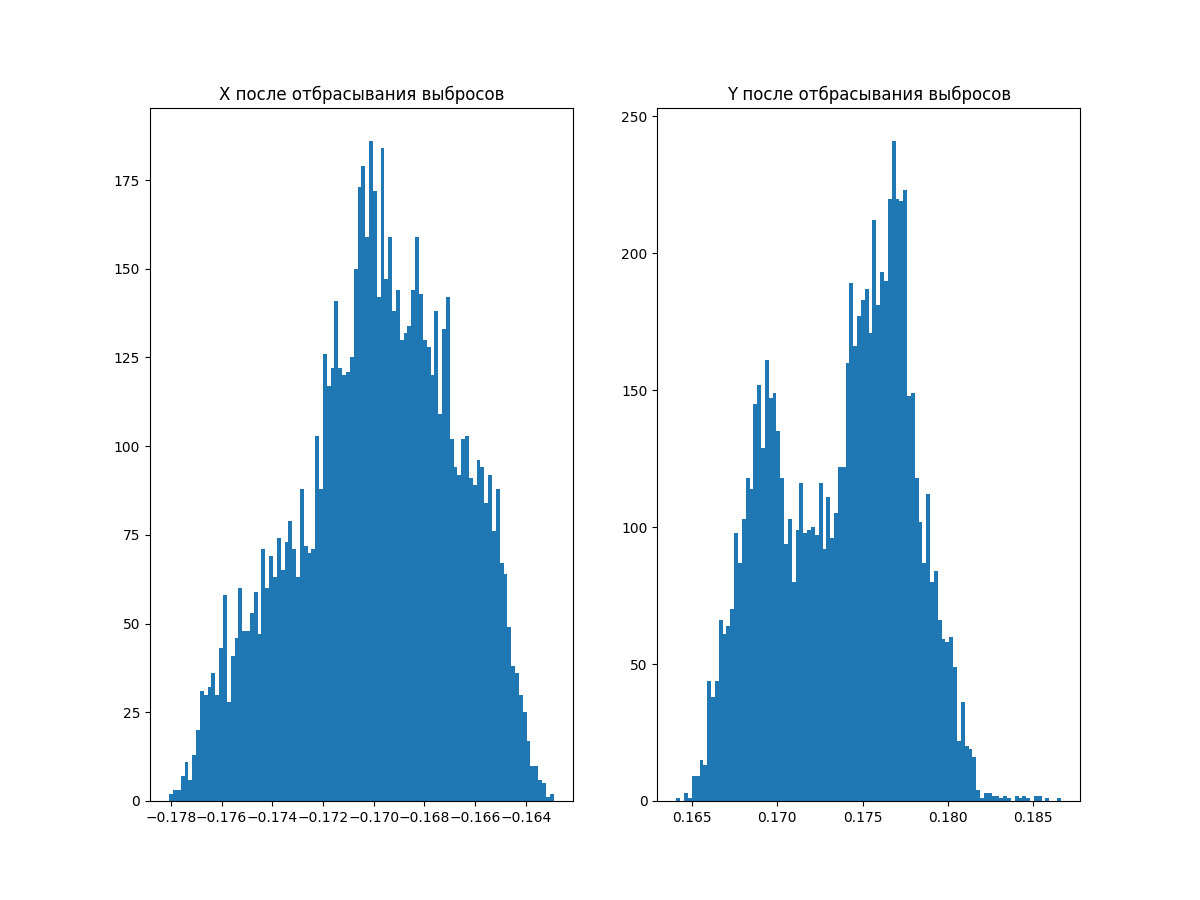
\includegraphics[width=0.7\linewidth]{XYafter.png}
    \caption{Изначальные данные (X и Y)}
\end{figure}
\begin{figure}[h!]
    \centering
    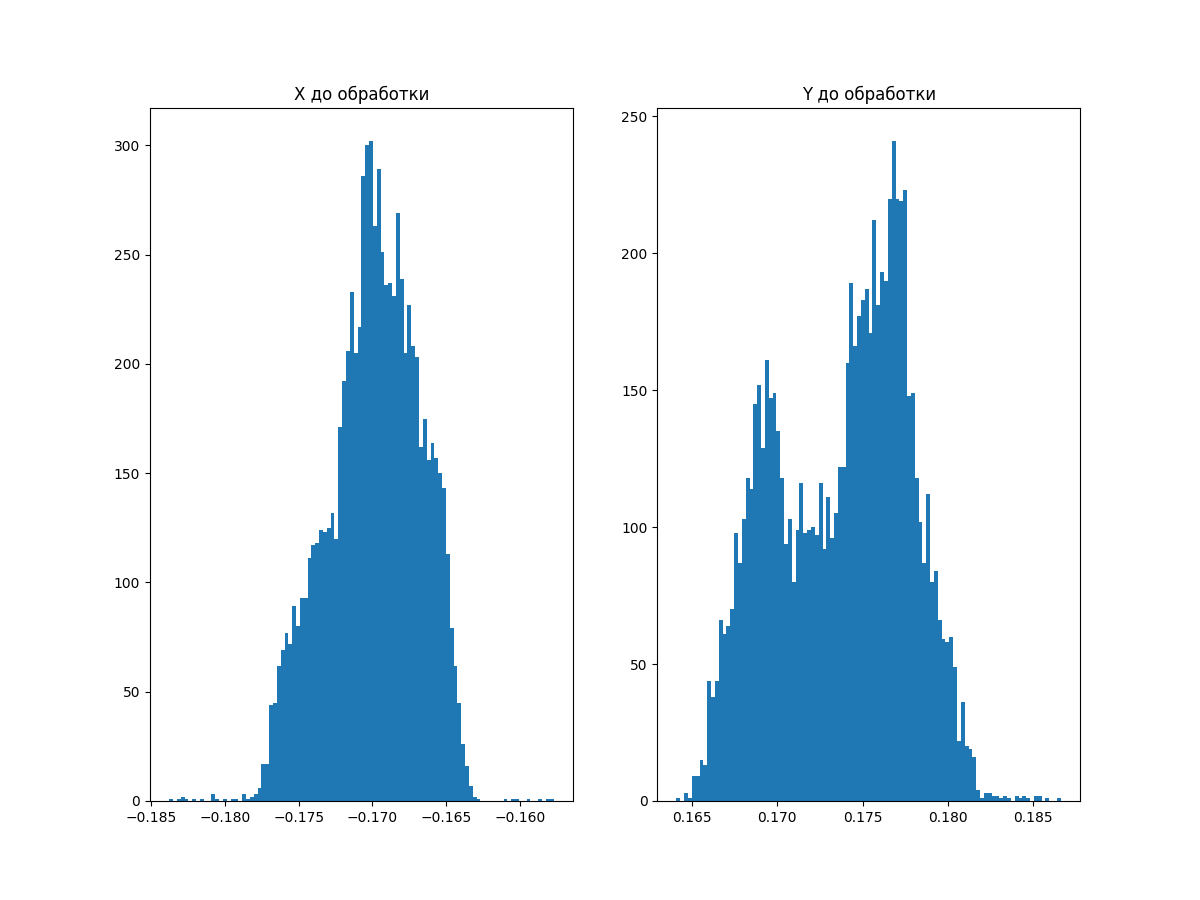
\includegraphics[width=0.7\linewidth]{XYbefore.png}
    \caption{Изначальные данные (X и Y) после устранения выбросов}
\end{figure}
\newpage
\begin{figure}[h!]
    \centering
    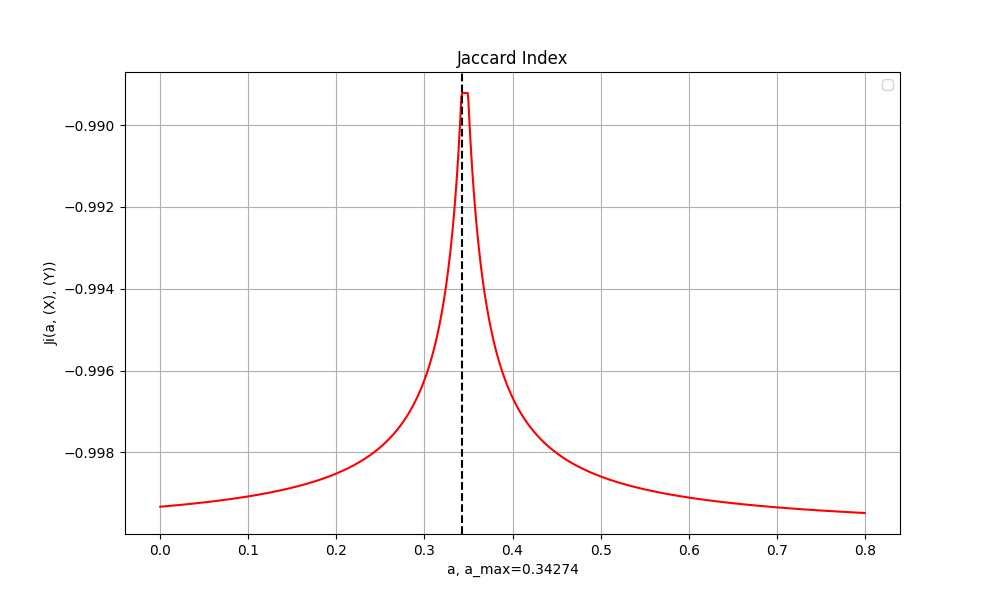
\includegraphics[width=0.9\linewidth]{Jaccard-a-.png}
    \caption{Коеффициент Жаккара для a, функционал (6)}
\end{figure}
\begin{figure}[h!]
    \centering
    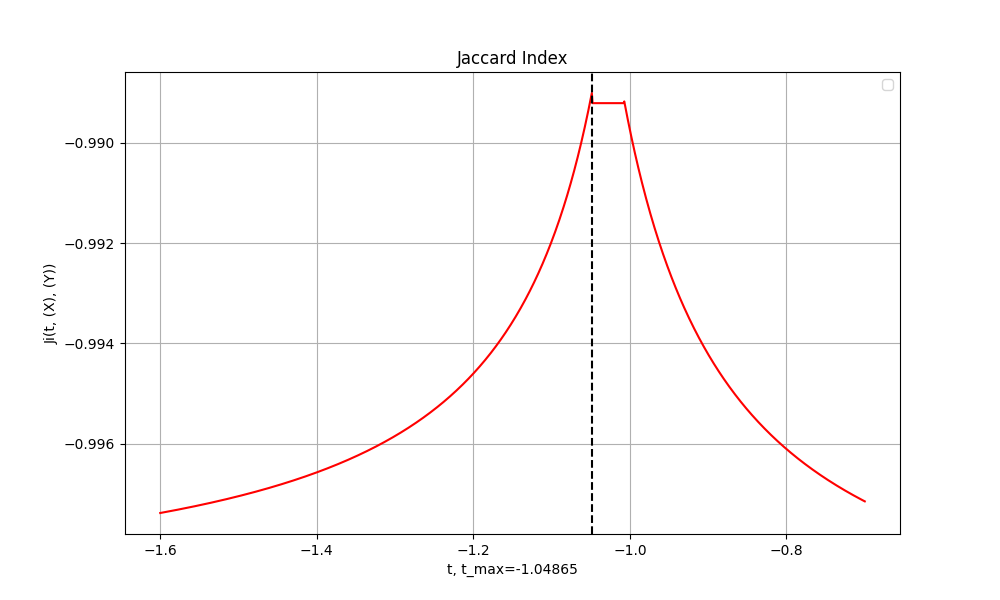
\includegraphics[width=0.9\linewidth]{Jaccard-t-.png}
    \caption{Коеффициент Жаккара для t, функционал (6)}
\end{figure}

\newpage
\begin{figure}[h!]
    \centering
    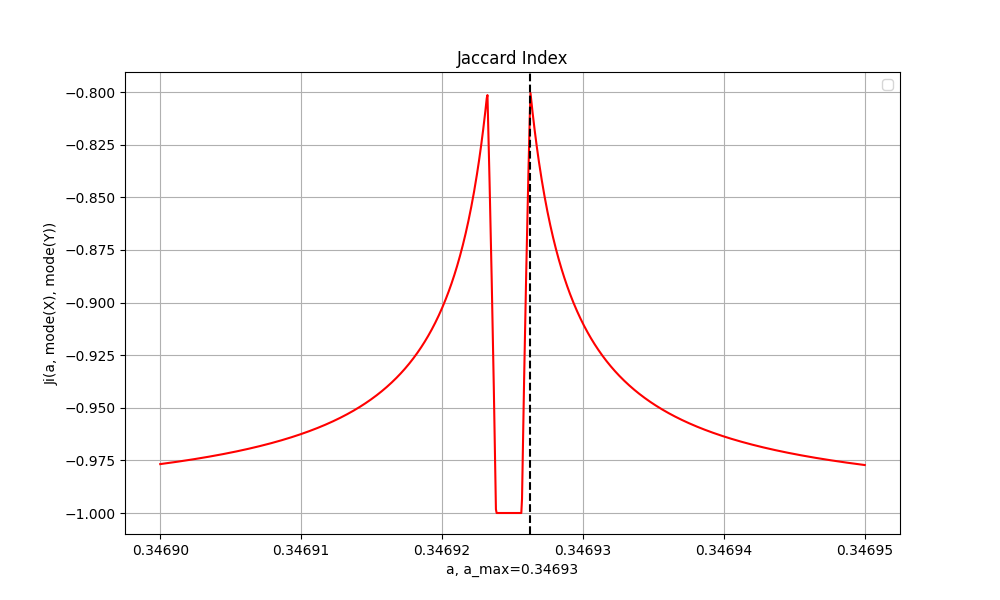
\includegraphics[width=0.9\linewidth]{Jaccard-a-mode.png}
    \caption{Коеффициент Жаккара для a, функционал (7)}
\end{figure}

\begin{figure}[h!]
    \centering
    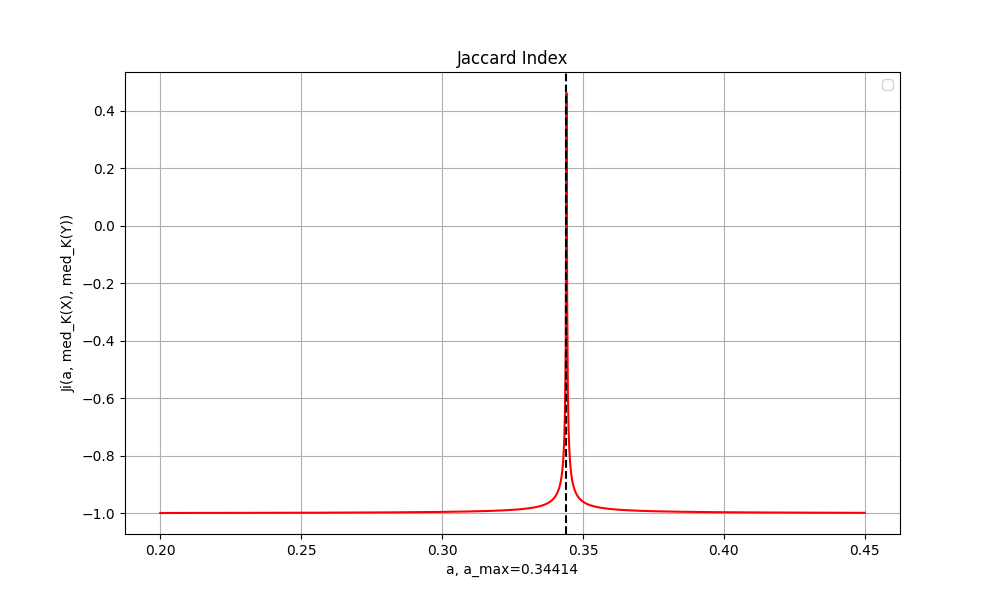
\includegraphics[width=0.9\linewidth]{Jaccard-a-med_K.png}
    \caption{Коеффициент Жаккара для a, функционал (8)}
\end{figure}

\newpage
\begin{figure}[h!]
    \centering
    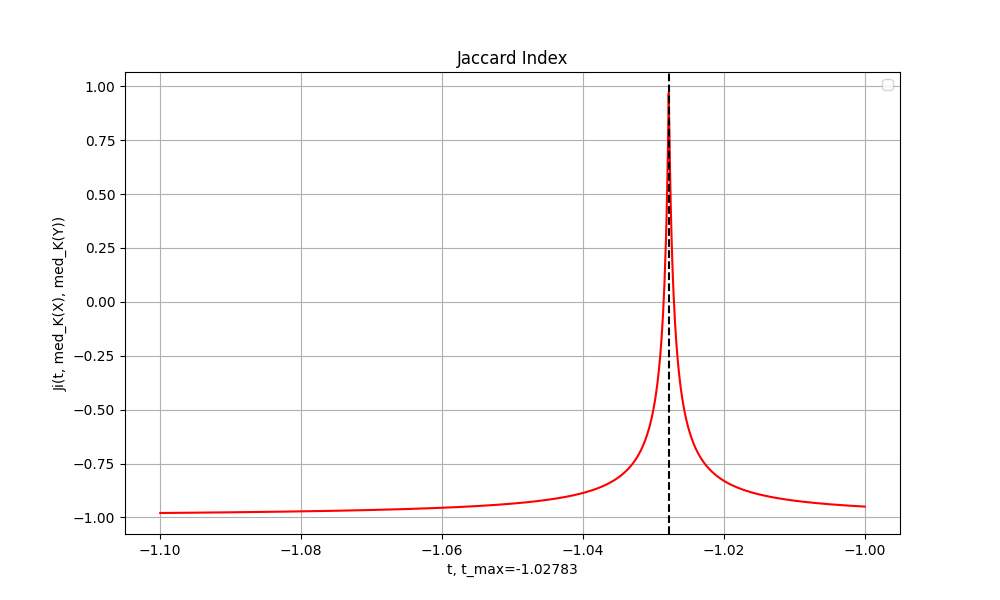
\includegraphics[width=0.9\linewidth]{Jaccard-t-med_K.png}
    \caption{Коеффициент Жаккара для t, функционал (8)}
\end{figure}

\begin{figure}[h!]
    \centering
    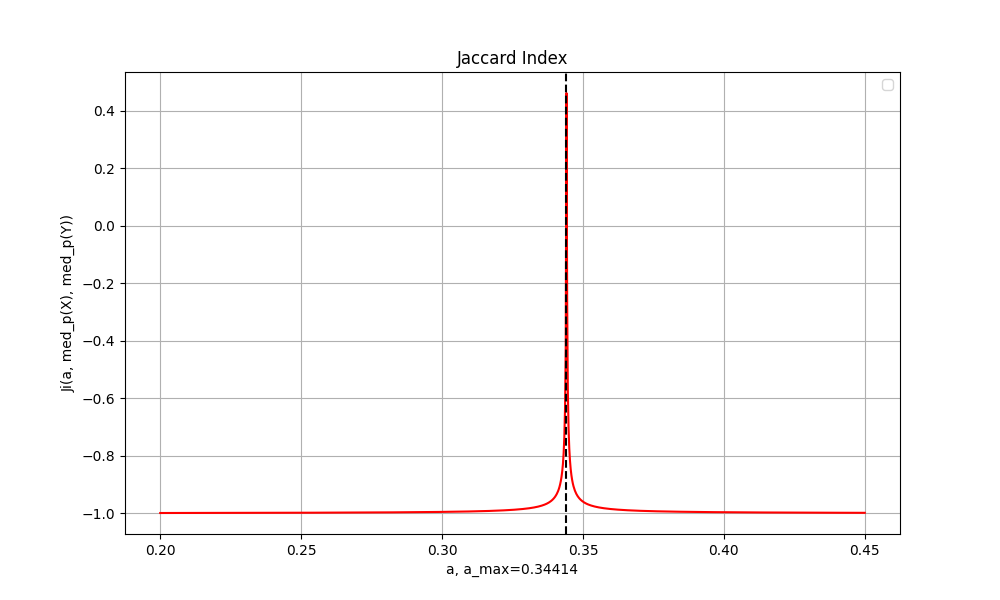
\includegraphics[width=0.9\linewidth]{Jaccard-a-med_p.png}
    \caption{Коеффициент Жаккара для a, функционал (9)}
\end{figure}

\newpage
\begin{figure}[h!]
    \centering
    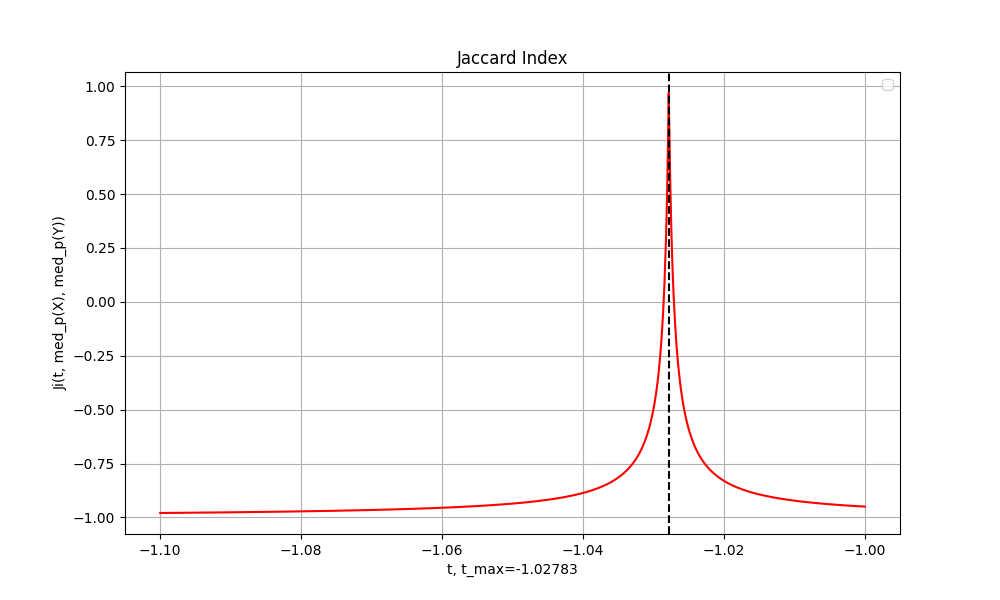
\includegraphics[width=0.9\linewidth]{Jaccard-t-med_p.png}
    \caption{Коеффициент Жаккара для t, функционал (9)}
\end{figure}

\newpage
\section{Выводы}
В ходе выполнения лабораторной работы познакомились со схемой получения интервальных оценок для констант. Для этого были использованы 4 разных функционала ((6), (7), (8), (9)), в основе которых лежит вычисление коэффициента Жаккара, но от разных интервальных множеств.\\
\\
Были деланы следующие выводы:
\begin{enumerate}
    \item Нужно аккуратно выбирать функционал, с помощью которого производится поиск оценки. Потому что в зависимости от того какой функционал выберем, множества интервалов, составленных в соответсвии с уравнениями (3), (4), могут оказаться несовместными, как это было получено при использовании функционала $Ji(const,\mathbf{X},\mathbf{Y})$; или наоборот оказаться совместными, как это было для функционалов: $\text{Ji} (const, \text{med}_K \mathbf{X}, \text{med}_K \mathbf{Y})$, $\text{Ji} (const, \text{med}_P \mathbf{X}, \text{med}_P \mathbf{Y})$.
    \item Можем заметить, что при использовании функционалов зависящих от медиан (8), (9), коэффициент Жаккара для оценки t достаточно близок к 1 (0.7746), что говорит о том, что две выборки $t*\mathbf{X}$ и $Y$ совместны и достаточно сильно совпадают.
    \item Также можем отметить, что при выборе функционала зависящего от моды (7), поиск оценок происходил намного дольше, чем для других функционалов. Что говорит нам о том, что для больших интервальных выборок лучше не использовать коэффициент Жаккара от интервальных мод (7), лучше будет выбрать коэффициент Жаккара от одной из медиан (Крейновича или Пролубникова).
    \item Можем отметить, что если при нахождении медианы Пролубникова ввести отношение порядка на алгебре \( \mathbb{IR} \) в центральном смысле (\( (\overline{\mathbf{a}} + \underline{\mathbf{a}}) / 2 \leq (\overline{\mathbf{b}} + \underline{\mathbf{b}}) / 2 \)), то оценки констант при использовании функционала от медианы Крейновича и при использовании функционала от медианы Пролубникова получились одинаковыми.
    
\end{enumerate}

\section{GitHub}
Ссылка на репозиторий с кодом: \url{https://github.com/11AgReS1SoR11/Interval.git} \\

\section{Литература}
\begin{enumerate}
    \item A.Н.Баженов. Интервальный анализ. Основы теории и учебные примеры. СПБПУ. 2020
    \item A.Н.Баженов., Н.В.Ермаков. Малоракурсная томография. Спб.: Политех-Пресс. 2023.  
\end{enumerate}

\end{document}
